%%%%%%%%%%%%%%%%%%%%%%%%%%%%%%%%%%%%%%%%%%%%%%%%%%%%%%%%
% Tech GreenHouse Node
% Copyright (C) 2016 Marco Giammarini
%
% Author(s):
%  Marco Giammarini <m.giammarini@warcomeb.it>
%
% This program is free software: you can redistribute it and/or modify
% it under the terms of the GNU General Public License as published by
% the Free Software Foundation, either version 3 of the License, or
% any later version.
%
% This program is distributed in the hope that it will be useful,
% but WITHOUT ANY WARRANTY; without even the implied warranty of
% MERCHANTABILITY or FITNESS FOR A PARTICULAR PURPOSE.  See the
% GNU General Public License for more details.
%
% You should have received a copy of the GNU General Public License
% along with this program. If not, see <http://www.gnu.org/licenses/>
%
% The compiled version of this file is licensed under the:
% Creative Commons Attribution-ShareAlike 4.0 International License
% To view a copy of the license, visit <http://creativecommons.org/licenses/by-sa/4.0
%%%%%%%%%%%%%%%%%%%%%%%%%%%%%%%%%%%%%%%%%%%%%%%%%%%%%%%
 
 \documentclass{standalone}

\usepackage{tikz}
\newcommand{\mysize}[1]{\footnotesize{\textbf{#1}}} 
\newcommand{\myssize}[1]{\tiny{\textbf{#1}}} 

\usetikzlibrary{calc}

%%%%%%%%%%%%%%%%%%%%%%%%%%%%%%%%%%%%%%%%%%%%%%%%%%%%%%%
% Metadata for block definitions
%%%%%%%%%%%%%%%%%%%%%%%%%%%%%%%%%%%%%%%%%%%%%%%%%%%%%%%
\def\tableblockcenter{2}
\def\tableblockwdth{4}

%\def\frdmnum{4}
%\def\frdmheight{\frdmnum * 0.5 +1.5}
\def\frdmheight{3}

\def\supplyheight{3}

\begin{document}

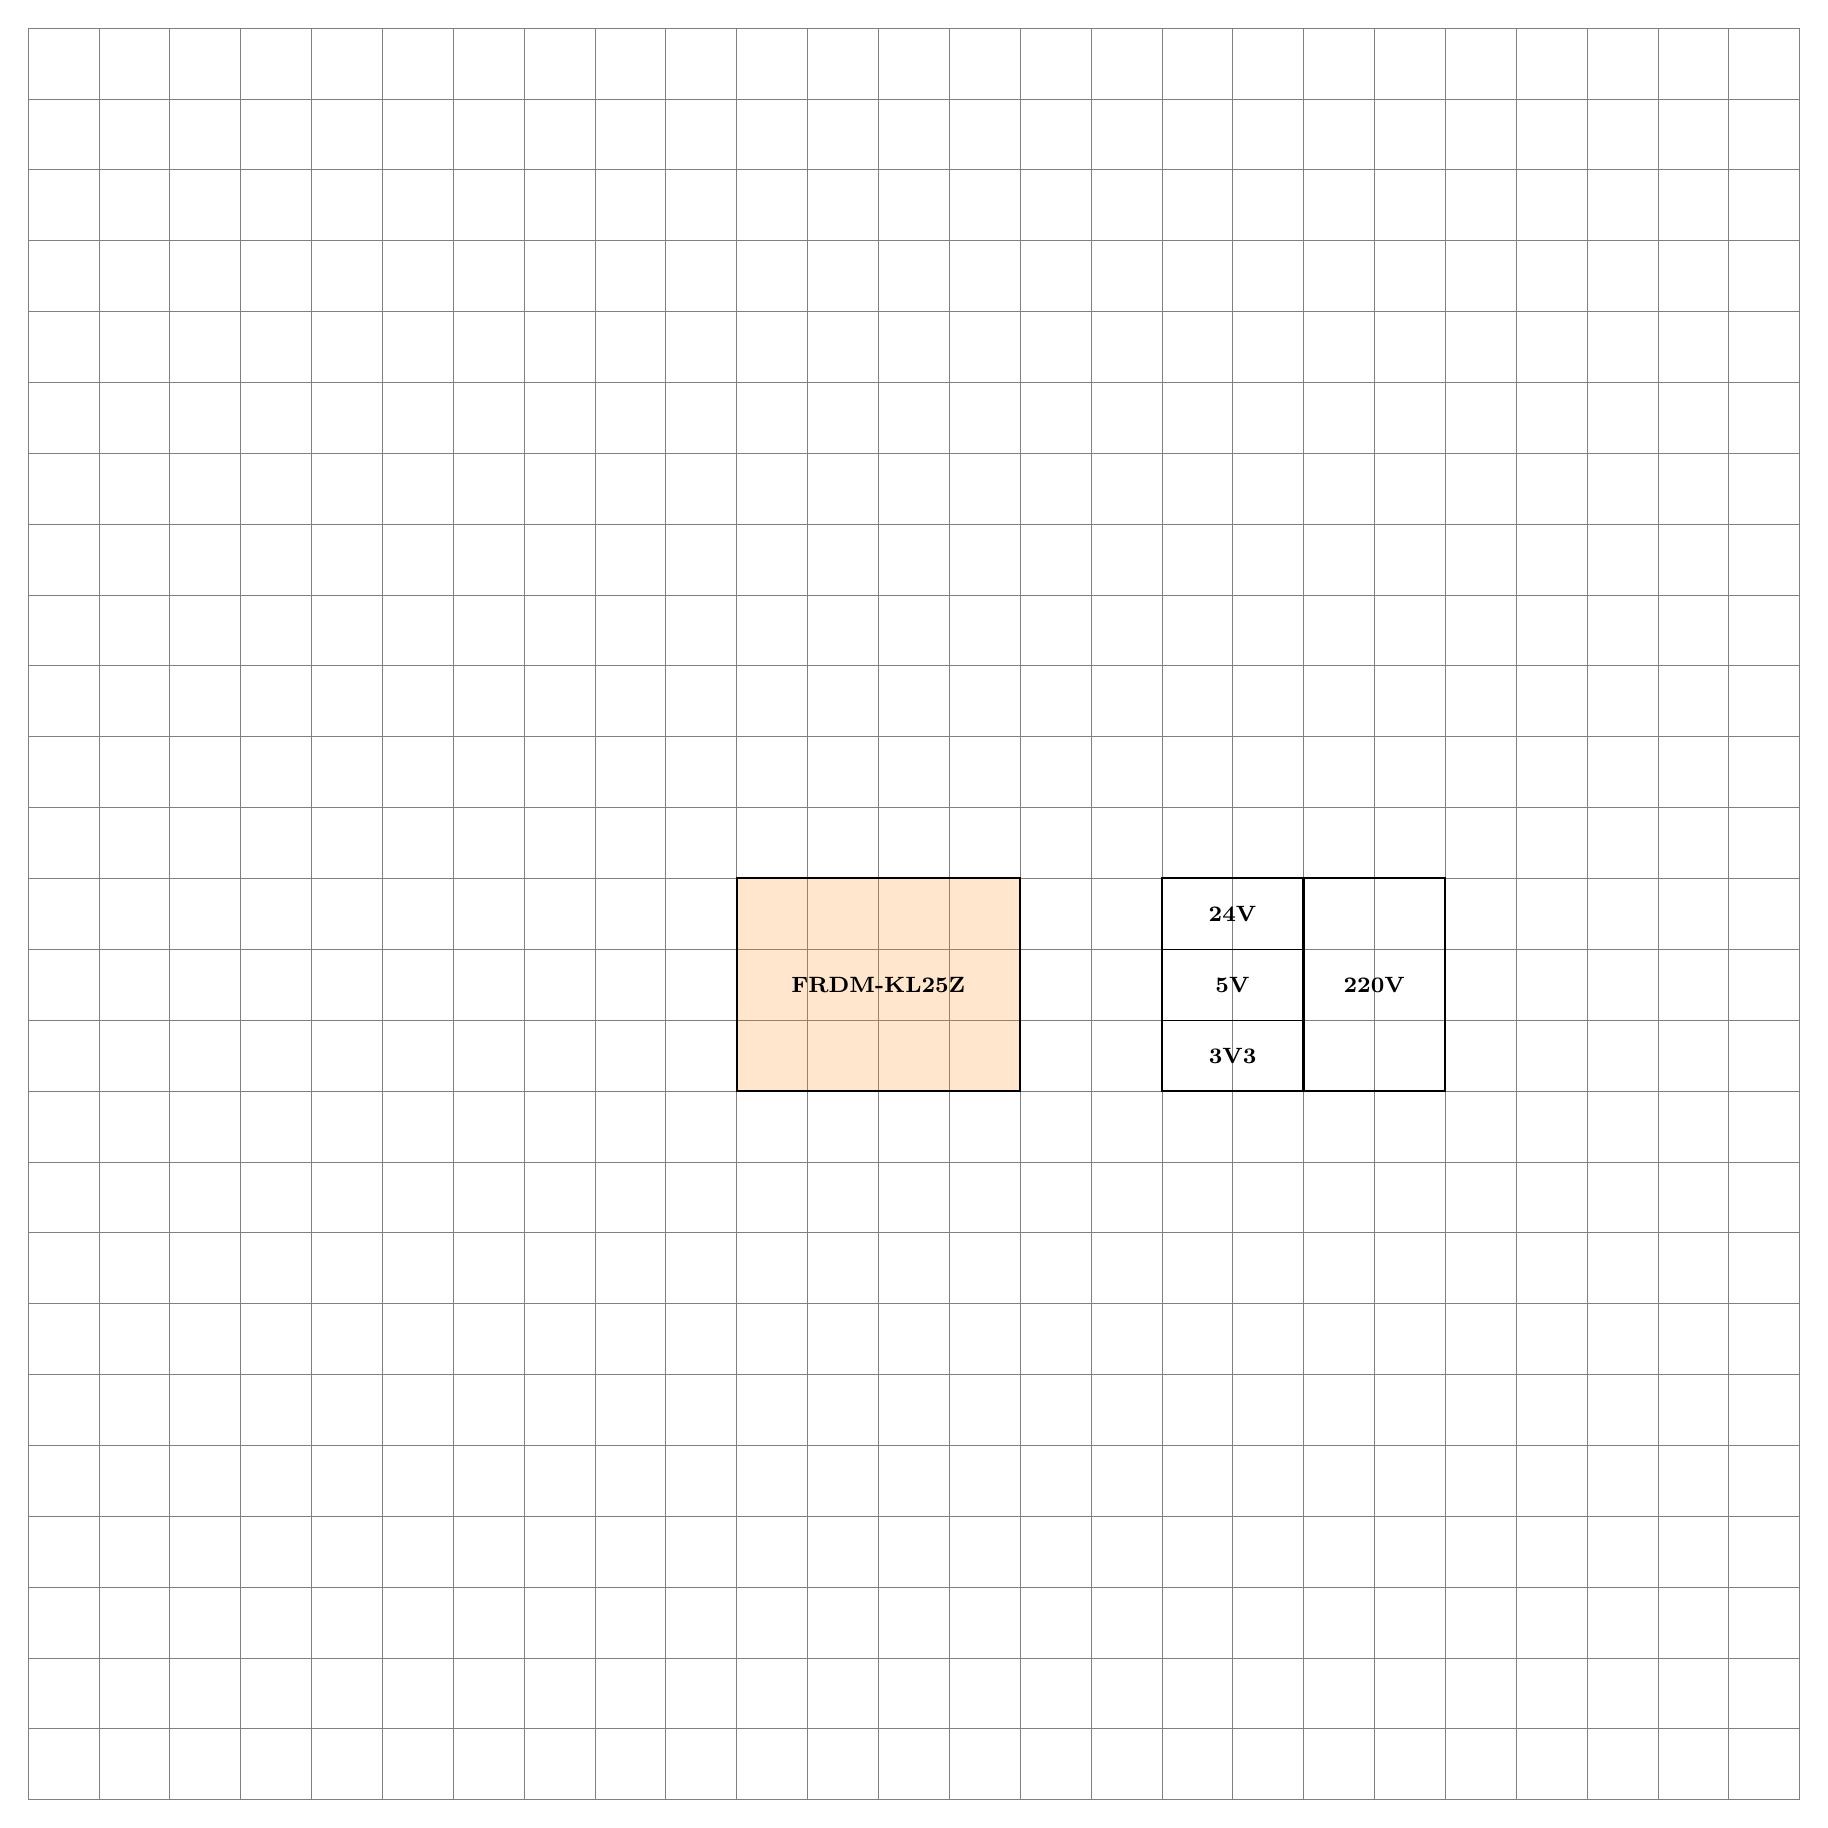
\begin{tikzpicture}[thick,scale=0.9]

\draw[help lines, style=gray] (0,0) grid (25,25);

% FRDM
\node (frdm) at (10,10){};
\draw [fill=orange, fill opacity=.2] (frdm) rectangle ($(frdm)+(\tableblockwdth , \frdmheight)$);
\node at ($(frdm)+(\tableblockcenter , \frdmheight/2)$) {\mysize{FRDM-KL25Z}};

% SUPPLY
\node (supply) at (16,10){};
\draw  (supply) rectangle ($(supply)+(\tableblockwdth , \supplyheight)$);
\draw  ($(supply)+(\tableblockwdth/2  , 0)$)--($(supply)+(\tableblockwdth/2 , \supplyheight)$);
\node at ($(supply)+(1 , \frdmheight/3 - 0.5)$) {\mysize{3V3}};
\draw[thin]($(supply)+(0  , \frdmheight/3)$)--($(supply)+(\tableblockwdth/2 ,\frdmheight/3)$);
\node at ($(supply)+(1 , \frdmheight/3 + 0.5)$) {\mysize{5V}};
\draw[thin]($(supply)+(0  , \frdmheight/3 + 1)$)--($(supply)+(\tableblockwdth/2 ,\frdmheight/3 + 1)$);
\node at ($(supply)+(1 , \frdmheight/3 + 1.5)$) {\mysize{24V}};
\draw[thin]($(supply)+(0  , \frdmheight/3 + 2)$)--($(supply)+(\tableblockwdth/2 ,\frdmheight/3 + 2)$);
\node at ($(supply)+(\tableblockwdth/2 + 1 , \frdmheight/2)$) {\mysize{220V}};
\end{tikzpicture}
\end{document}